\section{Results and discussion}\label{sec:results}


\todo[inline]{I think we can summarize the following paragraphs for a few sentences}

In this section, we detail the findings of our study.  We remind the reader that our main goal with this study is to observe the accuracy (false negative rate) of the state of the art in mining sandbox approaches using DroidBot, in the presence of a larger, representative dataset and shed light on a few of blindspots that impact the false negative rate. We hypothesize the presence of two blindspots - dynamic call trace from the entry point to a sensitive API, and the differences in the manifest file of repackaged apps. In Section~\ref{sec:Sensitive APIs}, we summarize the results of our study that estimates the performance of the state of the art in mining sandbox approaches. To this end, we reproduce the approach used by DroidBot in their original paper by presenting the divergent sensitive app sets for each app pair in our dataset. We also present details regarding which sensitive APIs are accessed more commonly with malwares. 
%We also present the 
%sensitive APIs set more injected by repackaged apps, among 162 explored. 
%We perform this initial study since it help solve our R1 and served as a reference to solve R2 and R3. \kn{How does this help solve R2 and R3.}

The remainder of this section is structured as follows. Section~\ref{sec:traceResults} presents the results of our study analyzing the impact of dynamic call trace on mining sandbox approaches, thereby answering R2. Section~\ref{sec:manifestResults} presents the results of our study analyzing the impact of modified manifest files on sandbox approaches, thereby answering R3. Section~\ref{sec:implications} presents some insights gained from the overall study and their potential implications.

\subsection{(Accuracy) False negative rate}\label{sec:Sensitive APIs}

In this section, we describe the results of reproducing the state-of-the-art Android sandbox approach on our new dataset of $800$ app pairs.
Firstly, given a pair of apps, we analyse each app version using the DroidBot test case generation tool with the DroidXP infrastructure. We repeat
every analysis three times for a period of three minutes.

After the three executions, DroidXP produces a dataset with the sensitive methods that both app versions call during each execution. We consider that a test
generation tool (DroidBot) could construct a sandbox able to detect a specific malware if there exists at least a call to a sensitive method that happens
only in the malicious version of the app. 
%This check is done using a Python script that compares the set of sensitive methods, called at both app versions (benign/malicious).

To this end, we use DroidXP to generate reports for each execution that includes a set of observations like the set of sensitive methods accessed by each app version (benign/malicious),
the sensitive methods accessed just by the malicious version (diff). If the set of sensitive methods accessed just by a malicious app is empty,
this implies that the sandbox approach for malware detection was not able to classify the malicious version as malign, leading to a false negative.

In the presence of our larger dataset of $800$ apps, DroidBot accurately classifies a total of $193$ ($24.12$\%) malware, presenting
at least one difference in the set of calls to sensitive APIs. The accuracy of the approach here is much lower in comparison to those reported by previous works---e.g.,
Bao et al. ($68$/$102$ - $66.66$\%)~\cite{DBLP:conf/wcre/BaoLL18} and Costa et al. ($73$/$96$ - $76.04$\%)~\cite{DBLP:journals/jss/CostaMMSSBNR22}. To ensure our experiments are not biased in anyway,
we reproduced the results using the same smaller datasets with $101$\footnote{At our work we could not execute 1 app pair from original dataset because of emulator compatibility} app pairs used in previous studies, and confirm accuracy percentages close to these previous works, ($64$/$101$ - $63.36$\%).
This indicates that when presented with a more representative dataset, the accuracy of mining sandbox approach using DroidBot drops significantly. 
%It is to be noted that
%the previous works used app pairs with a very high similarity score ($77\%$) \rb{I would not suggest that the similarity between the benign / malign versions of the apps might explain this difference,
%  since we already know the contrary} indicating most of their apps were similar to each other.  

Our exploration of all sensitive APIs called by all app pairs brought to the light the most frequently abused sensitive APIs that
appear in the repackaged, malicious version of the apps. We observed that when executed all 800 app pair, DroidBot called $75$ sensitive APIs at least one time (from our list of 162 sensitive APIs). Among them, $16$ APIs account for more than half of all calls ($51.06$\%).
%\rb{I could not understand the previous sentence}.
The sensitive API abused most by repackaged apps turned out to be \textbf{android.telephony.TelephonyManager: java.lang.String getDeviceId()}, which gets the device
IMEI\footnote{From Wikipedia: International Mobile Equipment Identity (IMEI) is a number, usually unique, to identify 3GPP and iDEN mobile phones.}.
Table~\ref{tab:APIused} presents the list of the most frequent sensitive APIs that only the malicious
version of the apps in our dataset call.

With these results, we observe that DroidBot suffers from a significantly low accuracy rate when presented with a representative dataset
(higher number of app pairs, more malware kinds and a diverse similarity index) 
%\rb{again, we should not put too much emphasis on similarity}, 
which encouraged us to endorse
efforts aimed at identifying potential blindspots with such approaches and eventually answering R2 and R3.



%\begin{landscape}
\begin{table*}[t]
 \scriptsize
  \caption{Sensitive APIs more used by repackage apps}
  \centering
  %\begin{small}
 \begin{tabular}{lc}

   \toprule
   Sensitive API & Occurrences \\
   \midrule
   01 android.telephony.TelephonyManager: java.lang.String getDeviceId() &  78 \\
   02 android.net.wifi.WifiManager: android.net.wifi.WifiInfo getConnectionInfo() &  64\\
   03 android.net.wifi.WifiInfo: java.lang.String getMacAddress() &  63 \\
   04 android.net.NetworkInfo: java.lang.String getTypeName() &  58 \\
   05 android.net.NetworkInfo: java.lang.String getExtraInfo() &  56 \\
   06 android.telephony.TelephonyManager: java.lang.String getSubscriberId() &  54 \\
   07 android.net.NetworkInfo: android.net.NetworkInfo State getState() &  52 \\
   08 android.database.sqlite.SQLiteOpenHelper: android.database.sqlite.SQLiteDatabase getWritableDatabase() &  49 \\
   09 android.database.sqlite.SQLiteDatabase: android.database.Cursor query(java.lang.String, ...,java.lang.String) &  47 \\
   10 android.telephony.TelephonyManager: java.lang.String getNetworkOperator() &  45\\
   11 android.telephony.TelephonyManager: android.telephony.CellLocation getCellLocation() &  44\\
   12 android.database.sqlite.SQLiteOpenHelper: android.database.sqlite.SQLiteDatabase getReadableDatabase() &  44\\
   13 android.telephony.gsm.GsmCellLocation: int getLac() &  42 \\
   14 android.telephony.gsm.GsmCellLocation: int getCid() &  42 \\
   
   15 android.net.ConnectivityManager: android.net.NetworkInfo getNetworkInfo(int) &  39 \\
   16 android.telephony.TelephonyManager: java.lang.String getNetworkOperatorName() &  36 \\
   .&  .\\
   .&  .\\
   .&  .\\
   74 android.app.ActivityManager: java.util.List getRecentTasks(int,int) & 1 \\
   75 android.net.NetworkInfo: java.lang.String toString() & 1 \\

 \bottomrule
                            Total & 1592 \\

 \end{tabular}
 %\end{small}
 \label{tab:APIused}
\end{table*}
%\end{landscape}

\begin{obs}{1}{}
   %\kn{Here we need to add some final take aways of the reproduction study}
   Our results indicate that in the presence of a representative dataset ($800$ app pairs as opposed to $102$ and a diverse similarity index), the accuracy of state of the art in mining sandbox approaches, using DroidBot drops significantly (from $63.36\%$ to $24.12\%$). Our results also indicate that only few sensitive APIs are responsible for majority of injected malware in repackaged apps. This encourages the emergence of new proposals that can support mine sandbox mitigating \textit{blindspot}s that lead to low accuracy.
 \end{obs}


%\kn{In this subsection, are we simply reproducing the results of existing papers. Because as far as I understand, tools like DroidBOT etc. were evaluated by simply comparing the sensitive APIs call. I am guessing here our contribution is to evaluate it on the larger dataset. I have given it a shot, please keep me posted if this is correct.}

\subsection{Trace Analysis Results}\label{sec:traceResults}

In this section, we describe the results of our investigation on how the trace from the entry point to sensitive API could impact the accuracy of sandbox approaches. Initially, we collect the call graphs of DroidBot execution using \emph{Logcat} and filter in the traces between the app's entry point and calls to any sensitive methods.

Then, using the callgraph from executions of both app versions (benign/malicious), we track the differences between their traces. We choose to investigate only app pairs that covered the same set of sensitive APIs detected in both versions during our first experiment (Section~\ref{sec:Sensitive APIs}). Our results show that among $607$ pair apps that had no difference between their sensitive APIs set, 176 of them ($29$\%) had different traces. This result provides evidence that the accuracy of sandbox approaches will be improved if the traces from entry point to sensitive APIs are considered.

It is to be noted that when made aware of the dynamic call trace, the accuracy of DroidBot with the original dataset with $101$ apps increases to $82.17\%$ ($83$/$101$) re-establishing that a trace analysis indeed benefits the accuracy of mining sandbox approaches. %\kn{Handrick, please add the full numbers in the table}

Table~\ref{tab:pa} summarizes the results of this investigation. The column \textbf{Same API set (SAPI)} shows the number of app pairs that had the same sensitive APIs explored at the first experiment, i.e, considered as undetected malware. The column \textbf{Trace Diff. (TD)} shows the number of app pairs (among the undetected ones) that have different traces from the entry point to the sensitive method. The column \textbf{Improv. \%} shows how much the malware detection of each tool could have been potentially improved if we considered the trace (calculated using ~\eqref{improve})

\begin{table}[ht!]
  \caption{Summary of the results of trace analysis. }
  \centering
  \begin{small}
 \begin{tabular}{lccc}
   \toprule
   Dataset&(SAPI) & Trace Diff.(TD) & Improv.(\%) \\   \midrule
   101 & 37 & 19 & 18.81 \\
   800 & 607 & 176 & 22 \\
 \bottomrule
 \end{tabular}
 \end{small}
 \label{tab:pa}
\end{table}



\begin{eqnarray}
Improvement & = & \frac{trace Diff. (TD) \times 100}{Total App Pairs Explored} 
\label{improve}
\end{eqnarray}


Figure~\ref{fig:maliciousTrace} shows an example of trace injected in the malicious version of the app \textbf{[com.android.remotecontrolppt]}. Here, benign and malicious app versions access the same sensitive method, \textit{getSubscriberid()}. This sensitive method returns the device's unique subscriber ID, and requires the manifest file permission "READ\underline{\space}PHONE\underline{\space}STATE", present in both app version. The original app accesses this method through $2$ traces (1 and 2), which suggests an expected action from app user. However, instead of the 2 original traces, the malicious version injected a third trace containing as an entry point a method that performs a stealth computation on a background thread, \textit{doInBackground}, suggesting an action without user's awareness.
%\fh{explain more about this example, and find another one }

\begin{figure}
\centering
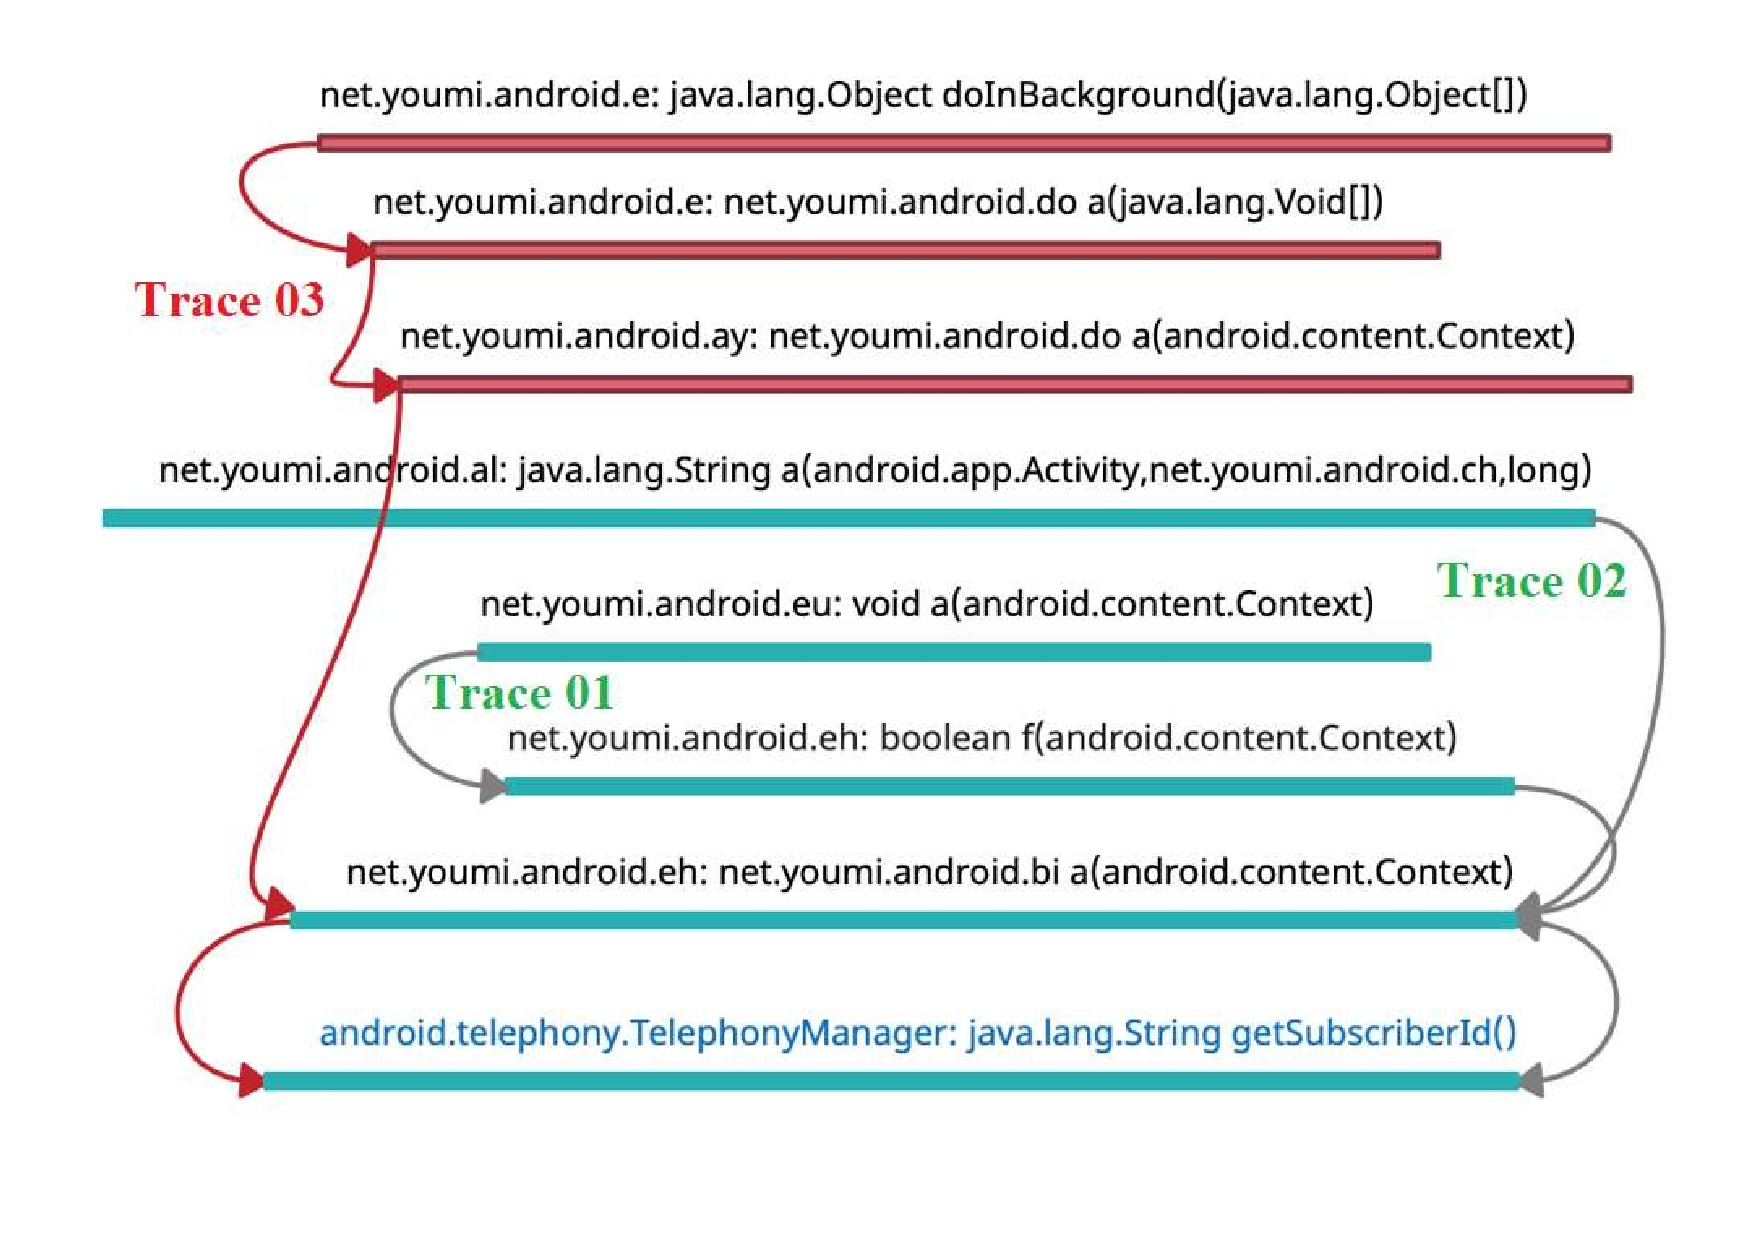
\includegraphics[scale=0.28]{images/maliciousTrace_example01.pdf}
\caption{Example of Malicious Trace.}
 \label{fig:maliciousTrace}
\end{figure}

\begin{obs}{2}{}
 The state of the art in mining sandbox approaches using DroidBot have a blind-spot when it comes to being aware of the trace taken from the entry point to a sensitive API call. The approaches could have a improvement of $22\%$ if it considered trace as a factor. Similar  improvements are also seen with the original dataset of $101$ app pairs (improvement of $18.81\%$).
 \end{obs}

\subsection{Manifest File Analysis}\label{sec:manifestResults}

In this section, we describe the results of our investigation on the impact of modified manifest files on the accuracy of sandbox approaches. 
To this end, we check some particulars from manifest file, that point to a likely suspicious behavior. In section \ref{sec:manifestAnalysis}, we illustrated that an automatic hacking script could inject permission requests at manifest file regardless of whether this request is already present on it, which can result in duplicated permission and actions in the Manifest file. We looked out for such modifications in the malware that went undetected by the test generation tools. Table~\ref{tab:mfa} summarizes our results.

\begin{table}[ht]
  \caption{Manifest File with duplicate code.}
  \centering
  \begin{small}
 \begin{tabular}{cccccc}
   \toprule
   Dataset & (SAPI) & (DP) & (DA) & (DP or DA) \\   \midrule
   101 & 37 & 7 & 12 & 17 \\ 
   800 & 607 & 62 & 81 & 120 \\ 
   
 \bottomrule
 \end{tabular}
 \end{small}
 \label{tab:mfa}
\end{table}

The column (SAPI) indicates the number of malware that went undetected during our first study (same as Table~\ref{tab:pa}'s Same API set (SAPI)). The second column (DP) indicates how many Manifest files from malicious app undetected at first study, had duplicated permission. Same way, column (DA) denotes the number of Manifest files with the duplicated actions in their manifest file.

A duplicate request for permission or action in a malicious version's manifest file should have been performed by a script. A simple analysis of manifest file could detect $120$ of undetectable malware from the first experiment ($607$), if it considers explorer duplicate permissions or actions at manifest file code as a detection strategy. If we combine the previous trace analysis with manifest file analysis, we improve the accuracy rate to $55.75\%$.

It is to be noted that in the presence of the original dataset of $101$ app pairs, the manifest file analysis combined with the trace analysis earlier discussed improves the accuracy rate to $90.09\%$ confirming that such an analysis, even though naive and simple does have an impact on the accuracy rate of mining sandbox approaches.  %\kn{Handrick as before please put the full numbers in the table}


\begin{obs}{3}{}
 We can conclude that sandbox approach also could have better accuracy if they considered the suspicious modifications in manifest file in their analysis. Although the analysis required of the manifest file is quite naive, we believe the results present an interesting and relevant insight for developers of malware detection tools to improve accuracy.
\end{obs}

\subsection{Insights}\label{sec:implications} \kn{This sounds more like summary of insights than potential implications}

The results presented so far have implications for both practitioners and researchers. We bring evidence that there are blindspots in Android sandbox approaches that if considered as a factor in malware identification, could improve sandbox techniques. In a first step, we present that in our study, the accuracy of sandboxes approach was significantly lower than presented in previous work. That is because our data set is almost $8$ times larger, encompasses a wider range of malware, and covers a diverse range of similarity index within the app pairs, all of which are not considered in previous works. Firstly, our study points out that when using DroidBot to explore sensitive APIs of both app versions, it was able to identify $193$ pairs where the set of sensitive APIs differ ($24.12$\%). We also show that among all sensitive APIs explored, \textbf{android.telephony.TelephonyManager: java.lang.String getDeviceId()} were the sensitive APIs most injected in repackaged malicious apps, responsible for $78$ calls among $1592$ observed in our experiment ($4.89\%$)

Next, we present a trace analysis which aimed to investigate whether there were different traces between an entry point and an access to any sensitive resource. Our findings indicate that the trace analysis is also effective for malicious apps identification, and could complement mining sandbox approaches. Among $607$ app pairs that were investigated, we observed that $176$ had different traces ($29\%$). The message from these findings is that exploring trace analysis in conjunction with mining sandbox approach is useful for researchers and practitioners to improve malicious app detection tasks. 

Finally, the last study used static analysis at Android manifest files, to investigate if even naive techniques to construct malicious apps can go unnoticed for mine sandbox approach. In the previous section, Table~\ref{tab:mfa} summarizes this investigation. Although manifest file analysis seems to be a simple technique, our results indicate that such an analysis on manifest files could have detected $120$ (more than one-third) of the undetected malware.

\textbf{Implications: }For industry and academia, these results have implications. They reinforce that there are benefits of integrating auxiliary techniques to mining sandbox approach for malware identification. 
%We also present evidence that its possible benefit from static analysis on suspicious Android manifest files for malware identification, even at malware with a low similarity coefficient regarding its benign version.
If we consider both integrated approaches, our accuracy rate in terms of malware detection grows from ($24.12\%$) to ($55.75\%$) in our representative dataset ($800$ app pair). %\kn{I donot understand the 22 and 9.63 here}

The Venn-diagram in Figure~\ref{fig:vennDiagram} presents the number of malicious app detected by the vanilla approach used in previous works, by trace analysis, and by two kinds of suspicious manifest files, as well as how they complement each other. As we can see, there are $114$ ($71+43$) samples detected just by the sensitive APIs diff approach. We can suppose that if malicious apps inject a new sensitive API at your repackage version, it also inserts a new Trace at this version. That is, samples identified by sensitive API diff should be a subset of the set of samples we identify by Trace diff approach. 

In that case, these malware samples were identified just by static analysis, which explored all sensitive APIs at app code. The samples do not have the opportunity of traces investigation of all sensitive APIs, since it just analysis traces from sensitive APIs explored by dynamic analysis. As described in Section~\ref{sec:pathsetup}, we use dynamic call graphs to investigate different access to sensitive APIs at both versions, and in that case, we do not have all dynamic call graphs of these samples. The interpretation of this result leads us to suppose that if the explorer tool used for dynamic analysis has a good code coverage, it can also explore more sensitive APIs and get more dynamic call graphs to investigate, which could result on accuracy improvement. In our experiment, $79$ ($41+38$) samples that injected new sensitive APIs at your malicious version, were also detected by Trace diff approach, since it naturally also inserted new traces at the code app. However, it's relevant to see that $176$ ($133+43$) samples were detected just by Trace diff approach, that is, it had the same sensitive APIs set explored at both versions, however had a different way to access them, which could mean a malicious call to sensitive API.


\begin{figure}[ht]
\centering
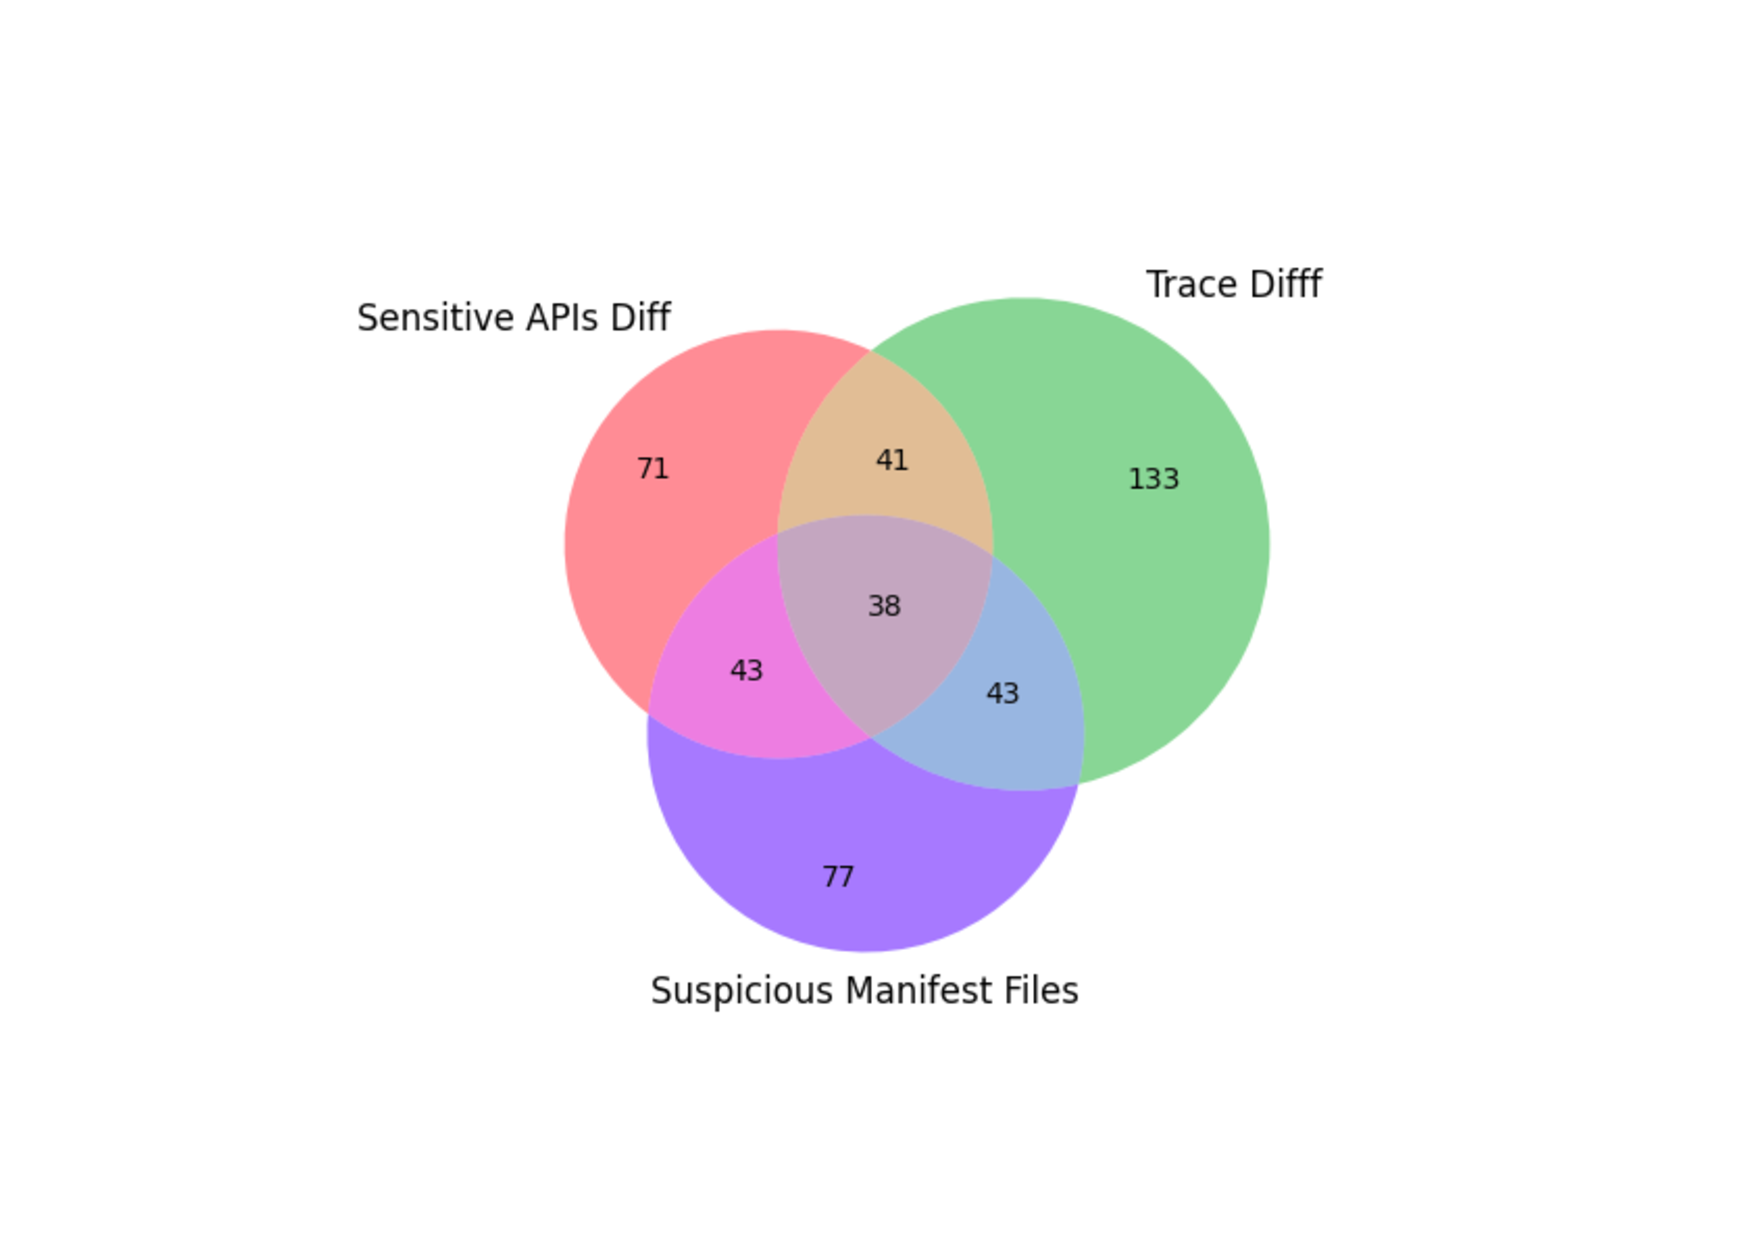
\includegraphics[scale=0.40]{images/vennDiagram.pdf}
\caption{Venn Diagram from results.}
 \label{fig:vennDiagram}
\end{figure}
